\providecommand{\pgfsyspdfmark}[3]{}

\documentclass[11pt,letterpaper]{article}
\usepackage[lmargin=1in,rmargin=1in,tmargin=1in,bmargin=1in]{geometry}

% -------------------
% Packages
% -------------------
\usepackage{
	amsmath,			% Math Environments
	amssymb,			% Extended Symbols
	enumerate,		    % Enumerate Environments
	graphicx,			% Include Images
	lastpage,			% Reference Lastpage
	multicol,			% Use Multi-columns
	multirow,			% Use Multi-rows
	gensymb
}


% -------------------
% Font
% -------------------
\usepackage[T1]{fontenc}
\usepackage{charter}
\usepackage{xcolor}

% -------------------
% Commands
% -------------------

\newcommand{\prob}{\noindent\textbf{Problem. }}
\newcounter{problem}
\newcommand{\problem}{
	\stepcounter{problem}%
	\noindent \textbf{Problem \theproblem. }%
}
\newcommand{\answer}{\noindent \textbf{Answer. }}
\newcommand{\pspace}{\par\vspace{\baselineskip}}
\newcommand{\ds}{\displaystyle}


% -------------------
% Header & Footer
% -------------------
\usepackage{fancyhdr}

\fancypagestyle{pages}{
	%Headers
	\fancyhead[L]{}
	\fancyhead[C]{}
	\fancyhead[R]{}
\renewcommand{\headrulewidth}{0pt}
	%Footers
	\fancyfoot[L]{}
	\fancyfoot[C]{}
	\fancyfoot[R]{}
\renewcommand{\footrulewidth}{0.0pt}
}
\headheight=0pt
\footskip=14pt

\pagestyle{pages}


% -------------------
% Content
% -------------------
\begin{document}
\noindent\textbf{\large Calculus I (AM\_\_1050AH / MSF\_10110) \\ 2022 Fall \\ Differentiation rules III, IV (Answer Key)}

\bigskip

\problem Find the following limits. You \textit{may} use L'Hôpital's rule \textit{if applicable}.
\begin{enumerate}[(a)]
    \item $\lim\limits_{x \to 1} \frac{\ln x}{\ln(x^3 + e^x)}$
    \item $\lim\limits_{x \to (-2)} \frac{\sin(\pi x)}{x^2-4}$
    \item $\lim\limits_{x \to \infty} \frac{x^2 + e^{4x}}{2x-e^x}$
    \item $\lim\limits_{x \to \infty} \frac{e^x-e^{-x}}{e^x+e^{-x}}$
    \item $\lim\limits_{x \to \infty} \sqrt[x]{x}$   (Hint: Show this is a $\infty^0$ form. Try evaluating the limit of its logarithm)
\end{enumerate}\vspace{6mm}

\answer
\begin{enumerate}[(a)]
    \item Plug-in method gets us $\frac{\ln 1}{\ln (1 + e)} = \frac{0}{\ln (1+e)} = 0$.
    \item Plug-in method gets us $\frac{0}{0}$ indeterminate form.  We can therefore use the L'Hôpital's rule: $\lim\limits_{x \to (-2)} \frac{\sin(\pi x)}{x^2-4} = \lim\limits_{x \to (-2)} \frac{[\sin(\pi x)]'}{(x^2-4)'} = \lim\limits_{x \to (-2)} \frac{\pi\cos(\pi x)}{2x} = \frac{\pi\cos(\pi(-2))}{2(-2)} = -\frac{\pi}{4}$.
    \item Divide $e^x$ from both the numerator and denominator and we get $\lim\limits_{x \to \infty} \frac{x^2 + e^{4x}}{2x-e^x} = \lim\limits_{x \to \infty} \frac{x^2e^{-x} + e^{3x}}{2xe^{-x}-1}$.  To use the plugin method, we need to evaluate $\lim\limits_{x \to \infty} x^2e^{-x}$ and $\lim\limits_{x \to \infty} xe^{-x}$, which are both $0$ (put $e^{x}$ to the denominator and use L'Hôpital's rule).  Therefore, the plug-in method yields $\frac{0+\infty}{0-1}$, which implies the limit goes to $-\infty$.
    \item Although the plug-in method indeed gets us $\frac{\infty}{\infty}$ in this case, using L'Hôpital's rule directly does not help.  To see this, $\lim\limits_{x \to \infty} \frac{(e^x-e^{-x})'}{(e^x+e^{-x})'} = \lim\limits_{x \to \infty} \frac{e^x+e^{-x}}{e^x-e^{-x}}$, which is still a $\frac{\infty}{\infty}$ indeterminate form.  Applying L'Hôpital's rule again and we yield $\lim\limits_{x \to \infty} \frac{(e^x+e^{-x})'}{(e^x-e^{-x})'} = \lim\limits_{x \to \infty} \frac{e^x-e^{-x}}{e^x+e^{-x}}$, which gets us to the original function!  To evaluate this limit, we will need common sense: $e^x$ seems to dominate $e^{-x}$ when $x$ goes to infinity, so we can try dividing $e^x$ from both the numerator and denominator, which yields $\lim\limits_{x \to \infty} \frac{e^x-e^{-x}}{e^x+e^{-x}} = \lim\limits_{x \to \infty} \frac{1-e^{-2x}}{1+e^{-2x}} = \frac{1-0}{1+0} = 1$.
    \item $\lim\limits_{x \to \infty} \sqrt[x]{x} = \lim\limits_{x \to \infty} x^{\frac{1}{x}} \text{(Plug-in gets } \infty^0 \text{)} = \lim\limits_{x \to \infty} e^{\ln (x^{1/x})} = \lim\limits_{x \to \infty} e^{\frac{\ln x}{x}} = e^{\lim\limits_{x \to \infty} \frac{\ln x}{x}}$.  Plug-in method on the exponent yields the $\frac{\infty}{\infty}$ indeterminate form, so we apply L'Hôpital's rule: $e^{\lim\limits_{x \to \infty} \frac{\ln x}{x}} = e^{\lim\limits_{x \to \infty} \frac{(\ln x)'}{(x)'}} = e^{\lim\limits_{x \to \infty} \frac{1/x}{1}} = e^0 = 1$. 
\end{enumerate}\vspace{6mm}

\noindent\begin{minipage}{0.7\textwidth}
    \problem Suppose we have $x^2+y^3=4$,
    \begin{enumerate}[(a)]
        \item Express $y$ as terms of $x$.
        \item Find $\frac{dy}{dx}$ using the expression in (a).
        \item Find $\frac{dy}{dx}$ using implicit differentiation on $x^2+y^3=4$.
        \item Show that the results in (b) and (c) are identical.
    \end{enumerate}
\end{minipage}
\begin{minipage}{0.3\textwidth}
    \begin{center}
        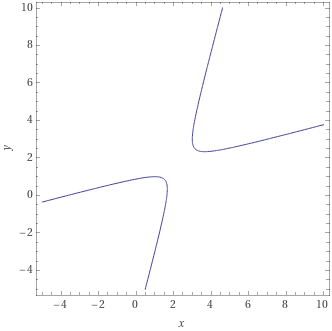
\includegraphics[width = \textwidth]{../graph/A09.png}
    \end{center}
\end{minipage}
\vspace{6mm}

\answer
\begin{enumerate}[(a)]
    \item $y^3 = 4-x^2 \Rightarrow y = \sqrt[3]{4-x^2}$
    \item $\frac{d}{dx}\sqrt[3]{\textcolor{red}{4-x^2}} = \frac{1}{3}\frac{1}{(\sqrt[3]{\textcolor{red}{4-x^2}})^2}(\textcolor{red}{4-x^2})' = -\frac{2x}{3(\sqrt[3]{4-x^2})^2}$
    \item Differentiating by $x$ at both sides and we yield $2x+(y^3)'=0$, where $(y^3)' = \frac{dy^3}{dy}y' = 3y^2y'$.  Therefore, $2x + 3y^2y' = 0 \Rightarrow y' = -\frac{2x}{3y^2}$
    \item Plugging $y = \sqrt[3]{4-x^2}$ into (c) and we yield $-\frac{2x}{3y^2} = -\frac{2x}{3(\sqrt[3]{4-x^2})^2}$, so (b) and (c) indeed yield identical results.
\end{enumerate}\vspace{6mm}

\problem A hyperbola $\Gamma$ on a Cartesian plane can be described as $\Gamma:x^2-4xy+y^2+2x+6y-6=0$, which is graphed above:
\begin{enumerate}[(a)]
    \item Find all points on $\Gamma$ that has $x$-coordinate of 1.
    \item Find the tangent line(s) of $\Gamma$ at the point(s) in (a).
    \item Find all tangent lines of $\Gamma$ that are horizontal.
    \item Find all tangent lines of $\Gamma$ that are vertical. (Hint: At where tangent lines are vertical, $\frac{dx}{dy} = 0$)
\end{enumerate}\vspace{6mm}

\answer
\begin{enumerate}[(a)]
    \item Suppose $(1, y_0)$ is on $\Gamma$, then from the equation for $\Gamma$, 
    \[1^2 - 4 \cdot 1 \cdot y_0 + y_0^2 + 2 \cdot 1 + 6 y_0 - 6 =0\]
    \[y_0^2 + 2y_0 -3 = 0\]
    \[(y_0 - 1)(y_0 + 3) = 0\]
    \[y_0 = 1 \text{ or } -3\]
    Therefore, $(1, 1)$ and $(1, -3)$ are the two points on $\Gamma$ that have $x$-coordinate of $1$. 
    \item We have the points that the tangent lines pass through, so now we obtain their slopes with implicit differentiation, differentiating both side of the equation of $\Gamma$ by $x$ (denoting $()'$ as differentiation with respect to $x$):
    \begin{gather*}
        \left[x^2-4xy+y^2+2x+6y-6\right]' = 0\\
        2x - 4(xy)' + (y^2)' + 2 + 6y' = 0\\
        2x - 4[(x)'y + x(y)'] + 2yy' + 2 + 6y' = 0\\
        2x - 4y - 4xy' + 2yy' + 2 + 6y' = 0\\
        y' = \frac{x-2y+1}{2x-y-3} \quad \text{(when } 2x-y-3 \ne 0 \text{)}
    \end{gather*}
    Therefore, the slope of the tangent line through $(1, 1)$ is $\frac{1-2+1}{2-1-3} = 0$, so the equation of it is $y = 1$.  
    
    The slope of the tangent line through $(1, -3)$ is $\frac{1+4+1}{2+3-3} = 3$, so the equation of it is $y+3 = 3(x-1)$, i.e. $y = 3x - 6$.
    \item Suppose a tangent line of $\Gamma$ over point $(x_0, y_0)$ on $\Gamma$ is horizontal. Since the tangent line is horizontal, we have
    \begin{gather*}
        \left.\frac{dy}{dx}\right|_{(x, y)=(x_0, y_0)} = \frac{x_0-2y_0+1}{2x_0-y_0-3} = 0\\
        x_0-2y_0+1 = 0 \\
        x_0 = 2y_0-1
    \end{gather*}
    Moreover, since $(x_0, y_0)$ is on $\Gamma$, we have $x_0^2-4x_0y_0+y_0^2+2x_0+6y_0-6 = 0$.  Substituting $x_0$ with $2y_0 - 1$ and we yield:
    \begin{gather*}
        (2y_0-1)^2 - 4(2y_0-1)y_0 + y_0^2 + 2(2y_0-1)+6y_0-6 = 0\\
        -3y_0^2+10y_0-7 = 0\\
        -(y_0-1)(3y_0-7) = 0\\
        y_0 = 1 \text{ or } \frac{7}{3}
    \end{gather*}
    Therefore, we have two horizontal tangent lines that passes through points with $y$-coordinates of $1$ and $\frac{7}{3}$, respectively.  Their equations are then $y = 1$ and $y=\frac{7}{3}$.
    \item We may differentiate the equation of $\Gamma$ by $y$ at both sides and yield 
    \[\frac{dx}{dy}=\frac{2x-y-3}{x-2y+1} \quad \text{(when } x-2y+1 \ne 0 \text{)}\]
    Suppose a tangent line of $\Gamma$ over point $(x_0, y_0)$ on $\Gamma$ is vertical. Since the tangent line is vertical, we have
    \begin{gather*}
        \left.\frac{dx}{dy}\right|_{(x, y)=(x_0, y_0)} = \frac{2x_0-y_0-3}{x_0-2y_0+1} = 0\\
        2x_0-y_0-3 = 0 \\
        y_0 = 2x_0-3
    \end{gather*}
    Moreover, since $(x_0, y_0)$ is on $\Gamma$, we have $x_0^2-4x_0y_0+y_0^2+2x_0+6y_0-6 = 0$.  Substituting $y_0$ with $2x_0 - 3$ and we yield:
    \begin{gather*}
        x_0^2 - 4x_0(2x_0-3) + (2x_0-3)^2 + 2x_0 + 6(2x_0-3)-6 = 0\\
        -3x_0^2+14x_0-15 = 0\\
        -(x_0-3)(3x_0-5) = 0\\
        x_0 = 3 \text{ or } \frac{5}{3}
    \end{gather*}
    Therefore, we have two vertical tangent lines that passes through points with $x$-coordinates of $3$ and $\frac{5}{3}$, respectively.  Their equations are then $x = 3$ and $x=\frac{5}{3}$.
\end{enumerate}\vspace{6mm}

\problem Evaluate the following high-order derivatives
\begin{enumerate}[(a)]
    \item $\frac{d^2}{dx^2}(e^{-x}\sin x)$
    \item $\frac{d^2}{dx^2}\ln(\ln x)$
    \item $\frac{d^6}{dx^6}(x^5 + 7x^4 + 3x^3 + 2x + 1)$
    \item $\frac{d^{10}}{dx^{10}} e^x$
    \item $\frac{d^{10}}{dx^{10}}\cos 2x$
\end{enumerate}\vspace{6mm}

\answer
\begin{enumerate}[(a)]
    \item $\frac{d^2}{dx^2}(e^{-x}\sin x) = \frac{d}{dx}[(e^{-x})'\sin x + e^{-x} (\sin x)'] = \frac{d}{dx}[-e^{-x}\sin x + e^{-x} \cos x] = \frac{d}{dx}[e^{-x} (\cos x-\sin x)] = (e^{-x})' (\cos x-\sin x) + e^{-x} (\cos x-\sin x)' = -e^{-x}(\cos x-\sin x)+e^{-x}(-\sin x - \cos x) = -2e^{-x}\cos x$
    \item $\frac{d^2}{dx^2}\ln(\textcolor{red}{\ln x}) = \frac{d}{dx} \Big[\frac{1}{\textcolor{red}{\ln x}}\cdot(\textcolor{red}{\ln x})'\Big] = \frac{d}{dx} \Big[\frac{1}{\textcolor{blue}{x\ln x}}\Big] = - \frac{1}{(\textcolor{blue}{x\ln x})^2}(\textcolor{blue}{x\ln x})' = -\frac{(x)'\ln x + x (\ln x)'}{(x \ln x)^2} = -\frac{\ln x + 1}{(x \ln x)^2}$
    \item The function is a degree-5 polynomial, which is less than the differentiation order, 6.  Therefore, the high-order derivative is $0$.
    \item The derivative of $e^x$ is still $e^x$, so no matter what the order of derivative is, we always get $e^x$.
    \item Using the chain rule, $\frac{d}{dx} \cos 2x = 2(-\sin 2x)$, $\frac{d^2}{dx^2} \cos 2x = \frac{d}{dx} 2(-\sin 2x) = 2^2 (-\cos 2x)$, $\frac{d^3}{dx^3} \cos 2x = \frac{d}{dx} 2^2(-\cos 2x) = 2^3 \sin 2x$, $\frac{d^4}{dx^4} \cos 2x = \frac{d}{dx} 2^3 \sin 2x = 2^4 \cos 2x$.  The pattern is the $n^{\text{th}}$ derivative has a coefficient of $2^n$, and the function behind rotates between $-\sin 2x, -\cos 2x,$ $\sin 2x, \cos 2x$ in order.  (One may use induction to prove this rigorously).  Therefore, $\frac{d^{10}}{dx^{10}} \cos 2x = -2^{10} \cos 2x$
\end{enumerate}\vspace{6mm}

% \problem Use the hinted linear approximations to approximate the following quantities:
% \begin{enumerate}[(a)]
%     \item $\tan 46 \degree$, approximating $\tan x$ at $x = 45 \degree$. (Note: You'll have to operate in radians) 
%     \item $\ln(1.01)$, approximating $\ln (1+x)$ at $x = 0$.
%     \item $\tan^{-1}0.99$, approximating $\tan^{-1} x$ at $x = 1$.
%     \item $\sqrt[4]{80}$, approximating $3\sqrt[4]{1+x}$ at $x = 0$.
%     \item $\frac{1}{0.99^3}$, approximating $\frac{1}{(1+x)^3}$ at $x = 0$.
% \end{enumerate}\vspace{6mm}

% \problem Find the following limits. You \textit{may} use the L'Hôpital's rule \textit{if applicable}.
% \begin{enumerate}[(a)]
%     \item $\lim\limits_{x \to 1} \frac{x^3+x^2+x-3}{x^3+2x^2+x-3}$
%     \item $\lim\limits_{x \to 0} \frac{e^{(3x^2+2x)}-1}{\sin(2x^2+3x)}$
%     \item $\lim\limits_{x \to 0} \frac{\sin (x^2)}{x \tan x}$
%     \item $\lim\limits_{x \to 0} x^2 \ln (x^2)$ \quad (Hint: Transform it into $\frac{\infty}{\infty}$ form)
%     \item $\lim\limits_{x \to 0} \frac{e^{-\frac{1}{x^2}}}{x^2}$ \quad (Hint: $\frac{0}{0}$ form can also be transformed into $\frac{\infty}{\infty}$ form)
% \end{enumerate}\vspace{4mm}

% \problem Determine if the following statements are true or false and explain. (You can just provide a counterexample if you determine them as false)
% \begin{enumerate}[(a)]
%     \item If $f'(x) = g'(x)$ (for all $x\in \mathbb{R}$), then $f(x) = g(x)$
%     \item If $f(1) = 0$, then $f'(1) = 0$
%     \item If $f'(x) = 0$ (for all $x\in \mathbb{R}$), then $f(x) = 0$
% \end{enumerate}\vspace{6mm}

% \problem Let $f(x) = \sqrt[4]{x} - \sqrt{x}$,
% \begin{enumerate}[(a)]
%     \item Find the tangent line of $f(x)$ at the point where $x=16$.
%     \item At which point(s) on $f(x)$ is its tangent line horizontal?
%     \item Is $f(x)$ differentiable at $x = 0$? Why?
% \end{enumerate}\vspace{6mm}

% \problem A ball is expanding with its radius $r$ as a function of time $t$: $r(t) = \sqrt{t} + 2, t \ge 0$
% \begin{enumerate}[(a)]
%     \item Find the rate its radius is growing at $t = 1$
%     \item Find the rate its surface area is growing at $t = 1$
%     \item Find the rate its volume is growing at $t = 1$
% \end{enumerate}\vspace{6mm}

\end{document}